% !TEX TS-program = XeLaTeX
%!TEX encoding = UTF-8 Unicode
%==================================================
%      PREAMBOLO e DICHIARAZIONI INIZIALI
%==================================================
\documentclass[10pt,oneside,a4paper]{article}

\usepackage[utf8]{inputenc} 
\usepackage[italian]{babel}
\usepackage[T1]{fontenc}
\usepackage{siunitx} %Inserisce automaticamente i dati con le unità  di misura correttamente formattate del SI (utilizzo: \SI{0.82}{m^2}, in generale \SI{misura con il punto decimale}{unità  di misura})
\sisetup{output-decimal-marker = {.}, separate-uncertainty = true, input-uncertainty-signs = \pm, detect-weight=true, detect-family=true} %per usare SI con il punto decimale
\usepackage{listings} %Per citare codice informatico formattandolo correttamente
\usepackage{amsmath,amsthm,verbatim,amssymb,amsfonts,amscd,graphicx,mathtools}
\usepackage[makeroom]{cancel}
\newcommand{\abs}[1]{\left\lvert\,#1\,\right\rvert}
\usepackage{geometry}
\usepackage{epigraph}
\usepackage{booktabs}	%tabelle migliorate
\usepackage{tablefootnote}	%note a piè di pagina in tabella
\usepackage{threeparttable} %tabella con note a piè di tabella
\usepackage{caption}	%descrizione per figure
\usepackage{dblfnote}
\captionsetup{tableposition=top,figureposition=bottom,font=small} %setup descrizione
\usepackage{float}
\usepackage{esvect} %vettori
\usepackage{longtable} %tabelle lunghe
\usepackage[dvipsnames]{xcolor}
\definecolor{sepia}{HTML}{80002A}
\usepackage[colorlinks=true, citecolor=black, linkcolor=sepia, urlcolor=black]{hyperref}
\usepackage{mathrsfs}
\usepackage{circuitikz}
\tikzset{
  font={\fontsize{7pt}{12}\selectfont}}
\ctikzset{bipoles/resistor/height=0.2}
\ctikzset{bipoles/resistor/width=0.4}
\ctikzset{bipoles/diode/height=0.3}
\ctikzset{bipoles/diode/width=0.3}
\ctikzset{tripoles/american nand port/height=0.7}
\ctikzset{tripoles/american nand port/width=0.8}
\usepackage{enumitem} %Liste senza spazi verticali
\setlist{noitemsep}
\usepackage{amsmath}
\usepackage{hyperref}
%\usepackage{pst-optexp} %Diagrammi ottici
\usepackage{physics} %Ambienti utili


\interfootnotelinepenalty=10000


\usepackage{multicol}
\newenvironment{Figure}
  {\par\medskip\noindent\minipage{\linewidth}}
  {\endminipage\par\medskip}

%\newcommand{\var}{\operatorname{var}}
%\newcommand{\cov}{\operatorname{cov}}


\usepackage{listings} %Per inserire codice
\lstdefinestyle{CStyle}{
    backgroundcolor=\color{backgroundColour},   
    commentstyle=\color{mGreen},
    keywordstyle=\color{magenta},
    numberstyle=\tiny\color{mGray},
    stringstyle=\color{mPurple},
    basicstyle=\footnotesize\ttfamily,
    breakatwhitespace=false,         
    breaklines=true,                 
    captionpos=b,                    
    keepspaces=true,                 
    numbers=left,                    
    numbersep=5pt,                  
    showspaces=false,                
    showstringspaces=false,
    showtabs=false,                  
    tabsize=2,
    language=C
}

\definecolor{color1}{RGB}{90,0,0} % Color of the article title and sections
\definecolor{color2}{RGB}{0,20,50} % Color of the boxes behind the abstract and headings
\definecolor{mGreen}{rgb}{0,0.6,0}
\definecolor{mGray}{rgb}{0.5,0.5,0.5}
\definecolor{mPurple}{rgb}{0.58,0,0.82}
\definecolor{backgroundColour}{rgb}{0.95,0.95,0.92}


%==================================================
%                  PRIMA PAGINA
%==================================================

\title{\textsc{\textbf{Esperienza 2}: Interferometro di Michelson}}
\author{\small{G. Galbato Muscio} \and \small{F. Ghimenti} \and \small{L. Gravina} \and \small{L. Graziotto}}
\date{11 Aprile 2019}

\begin{document}
	\begin{figure}
		\centering
		
\includegraphics[scale=0.5, trim={2.8cm 8.9cm 0 9cm}, clip]{logo.png}
	\end{figure}
	\maketitle
	\begin{center} 
		\fbox{{\fontsize{12pt}{8mm}\textsc{Gruppo D1-1}}} \\
	\end{center}
\hrule
\vfill
\renewcommand{\abstractname}{Abstract}
\begin{abstract}
Si studia la visibilità delle frange di interferenza di un laser HeNe\footnote{\url{https://www.dropbox.com/s/5aqzs2uykfi8lms/8-Coherence_function_He_Ne.pdf?dl=0}} mediante un interferometro di Michelson e si misura il tempo di coerenza $\tau_\mathrm{c}$ del laser.
\end{abstract}
\vfill
\tableofcontents %Indice
\newpage


\pagebreak


\begin{multicols}{2}
%==================================================
%             APPARATO STRUMENTALE
%==================================================
\section{Apparato strumentale}

Si utilizza un laser He-Ne di lunghezza d'onda $\lambda = \SI{632.8}{nm}$, montato su tavolo ottico. 

In serie al laser è posta un'iride, allo scopo di evitare l'ingresso nel laser dei fasci di ritorno, che ne perturberebbero il comportamento. Uno specchio riflette la luce uscente dell'iride nell'interferometro di Michelson, costituito da un beam splitter e due specchi; il fascio ricombinato viene poi allargato da una lente divergente prima di essere misurato dal fotodiodo.

Uno dei due specchi costituenti l'interferometro viene installato su una base fissa e appoggiato su un cristallo piezoelettrico, quest'ultimo è fatto espandere e contrarre attraverso un'onda triangolare di frequenza $f_\mathrm{rampa} = \SI{2.016}{\hertz}$ e ampiezza $A_\mathrm{rampa} = \SI{20.8}{\volt}$; l'altro viene fatto traslare su un piano forato con distanza tra i fori pari a $d = \SI{2.50 \pm 0.01}{cm}$. 

La configurazione utilizzata è illustrata in Figura~\ref{fig:diagram}.

\begin{Figure}
	\begin{center}
	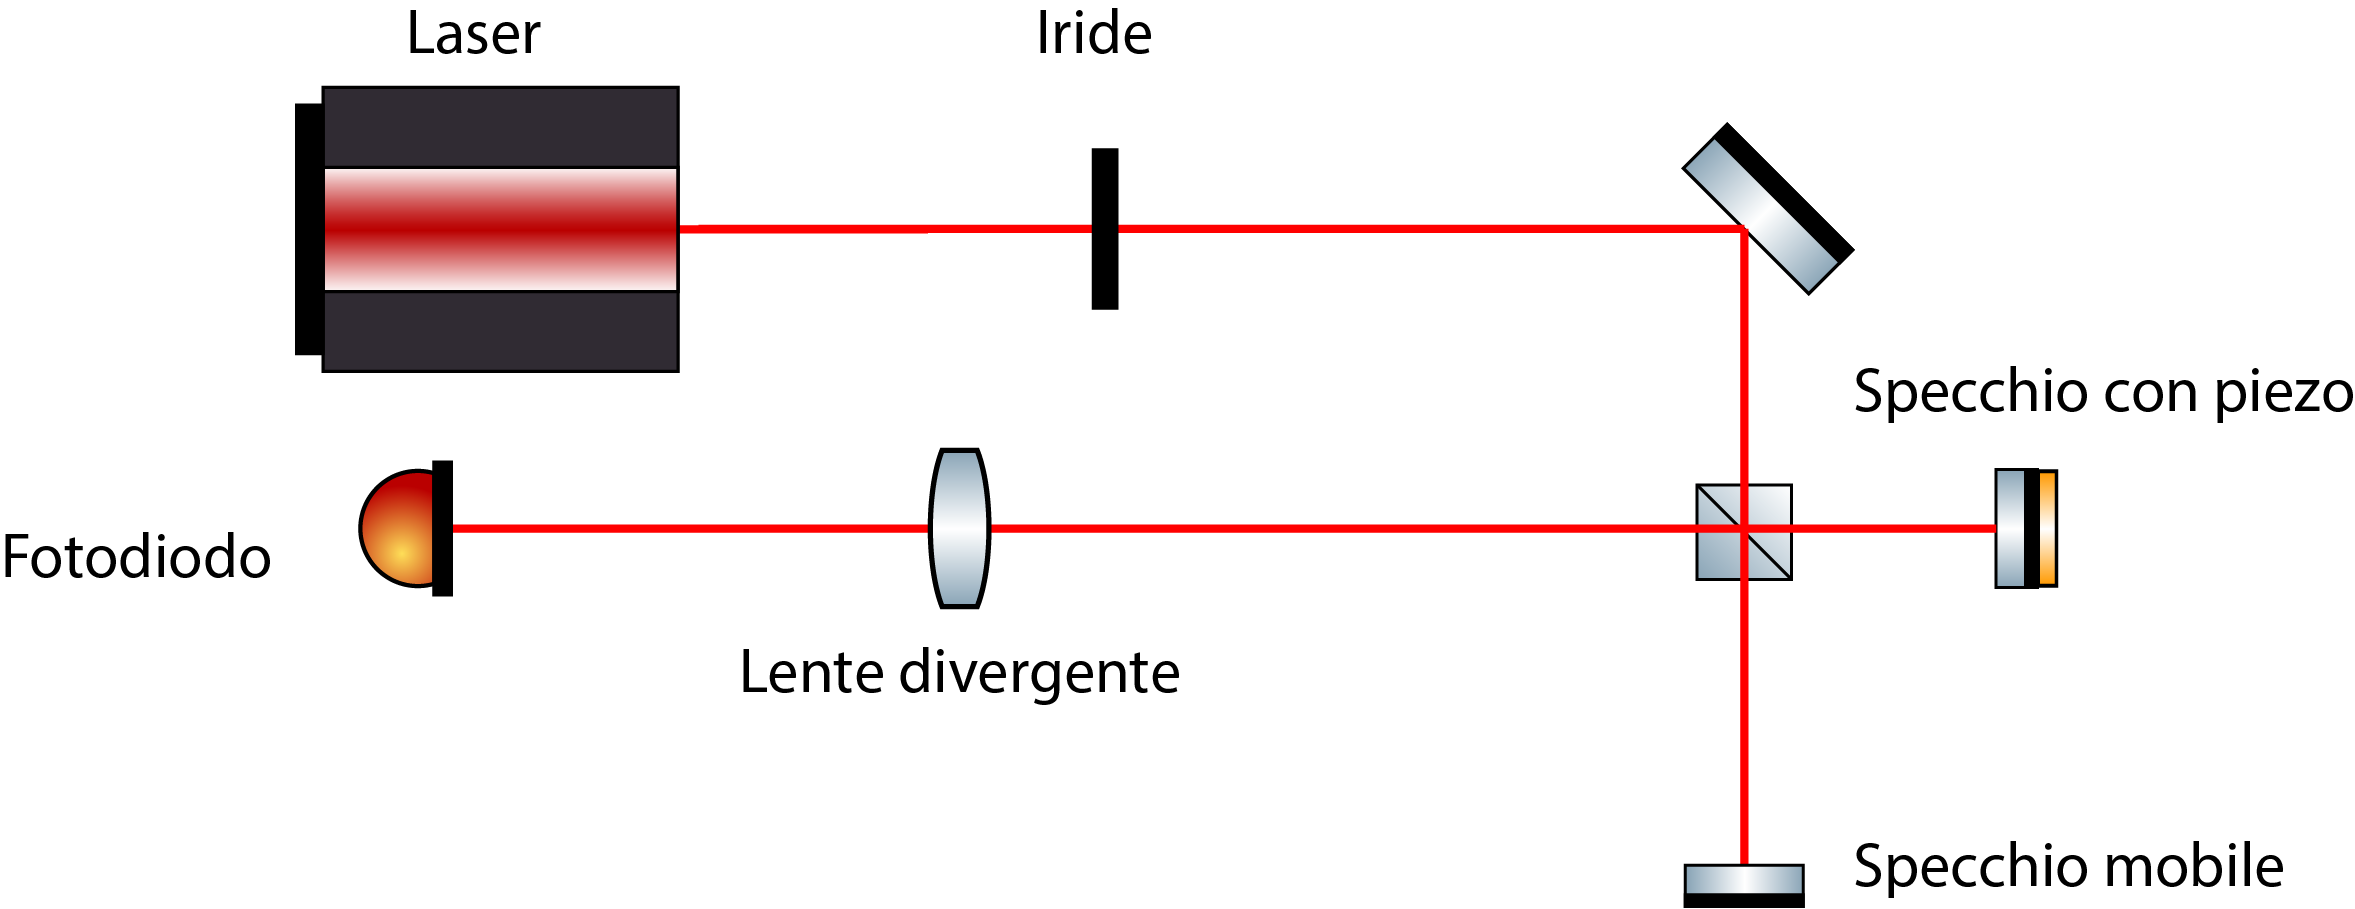
\includegraphics[width=\linewidth]{diagram.png}
	\captionof{figure}{Configurazione utilizzata.}
	\label{fig:diagram}
	\end{center}
\end{Figure}

Il segnale in uscita dal fotodiodo è misurato con l'oscilloscopio \texttt{Tektronik TDS2012C}, il cui trigger viene sincronizzato sulla frequenza del segnale uscente dal generatore. Le misure di intensità luminosa vengono riportate come differenza di potenziale misurata ai capi del fotodiodo, pertanto è da intendere la presenza di un fattore di proporzionalità non noto.

\section{Visibilità delle frange}
\subsection{Presa dati}
Si posiziona lo specchio mobile a distanza $d^{(0)}_\mathrm{mobile} = \SI{7.3 \pm 0.1}{cm}$, e quello fisso a distanza $d^{(0)}_\mathrm{fisso} = \SI{6.4 \pm 0.1}{cm}$, entrambe misurate rispetto all'interfaccia più prossima del beam splitter; si muovono gli specchi con l'utilizzo di viti micrometriche per collimare i due fasci riflessi al fine di massimizzare la visibilità percepita delle frange di interferenza e centrare il fascio allargato dalla lente sul fotodiodo. Sull'oscilloscopio si osserva l'intensità del fascio uscente dall'interferometro; essa mostra un andamento sinusoidale, caratteristico delle frange di interferenza; in particolare, la sinusoide è interrotta ad ogni cambio di pendenza dell'onda triangolare, poiché il cristallo piezoelettrico reagisce con una certa inerzia al segnale di input. Si misura quindi l'intensità massima $I_\mathrm{max}$ e minima $I_\mathrm{min}$ all'interno di una singola rampa (indifferentemente di salita o di discesa) dell'onda triangolare, utilizzando i cursori dell'oscilloscopio. 

Questa sequenza di operazioni viene ripetuta per tre volte, correggendo prima di ogni acquisizione sperimentale l'allineamento dei raggi; inoltre, prima di ogni ripetizione si misura l'intensità del fondo ambientale, che viene sottratta al dato acquisito, e la cui incertezza viene sommata in quadratura a quella strumentale. Quindi lo specchio mobile è spostato ad una distanza $d(N) = d^{(0)}_\mathrm{mobile} + Nd$, dove $N$ è il numero di fori liberi contati tra la base del beamsplitter e quella dello specchio mobile, mentre $d$ è la distanza interforo riportata in precedenza.
L'insieme di misure prese è riportato in Tabella \ref{tab:intensita}, in Appendice.

In seguito alle misure, ne viene effettuata un'ultima riavvicinando lo specchio mobile a distanza $d_\mathrm{mobile} = \SI{5.6 \pm 0.1}{cm}$ dal beamsplitter; in questo modo si acquisisce un ulteriore punto sperimentale per una differenza di cammino ottico minore.

L'incertezza associata alla misura della differenza di potenziale mediante i cursori è quella fornita dal manuale\footnote{\url{http://pdf1.alldatasheet.com/datasheet-pdf/view/554089/ETC2/TDS2012C.html}} dell'oscilloscopio, ossia il $3\%$.

\subsection{Analisi}
Si riportano in Figura~\ref{fig:averageIntensities} le medie con associate le incertezze (date dalla somma in quadratura di incertezza strumentale e dispersione statistica) dei tre valori di intensità massima e minima misurati per ogni fissata distanza tra specchi e beamsplitter\footnote{L'intensità del fondo è già sottratta, e l'incertezza dovuta a tale misura è sommata in quadratura e quindi inclusa in quella strumentale citata precedentemente.}, in funzione della differenza di cammino ottico $x = 2\cdot \left(d^{(0)}_\mathrm{fisso} - d(N)\right)$.

\begin{Figure}
	\begin{center}
	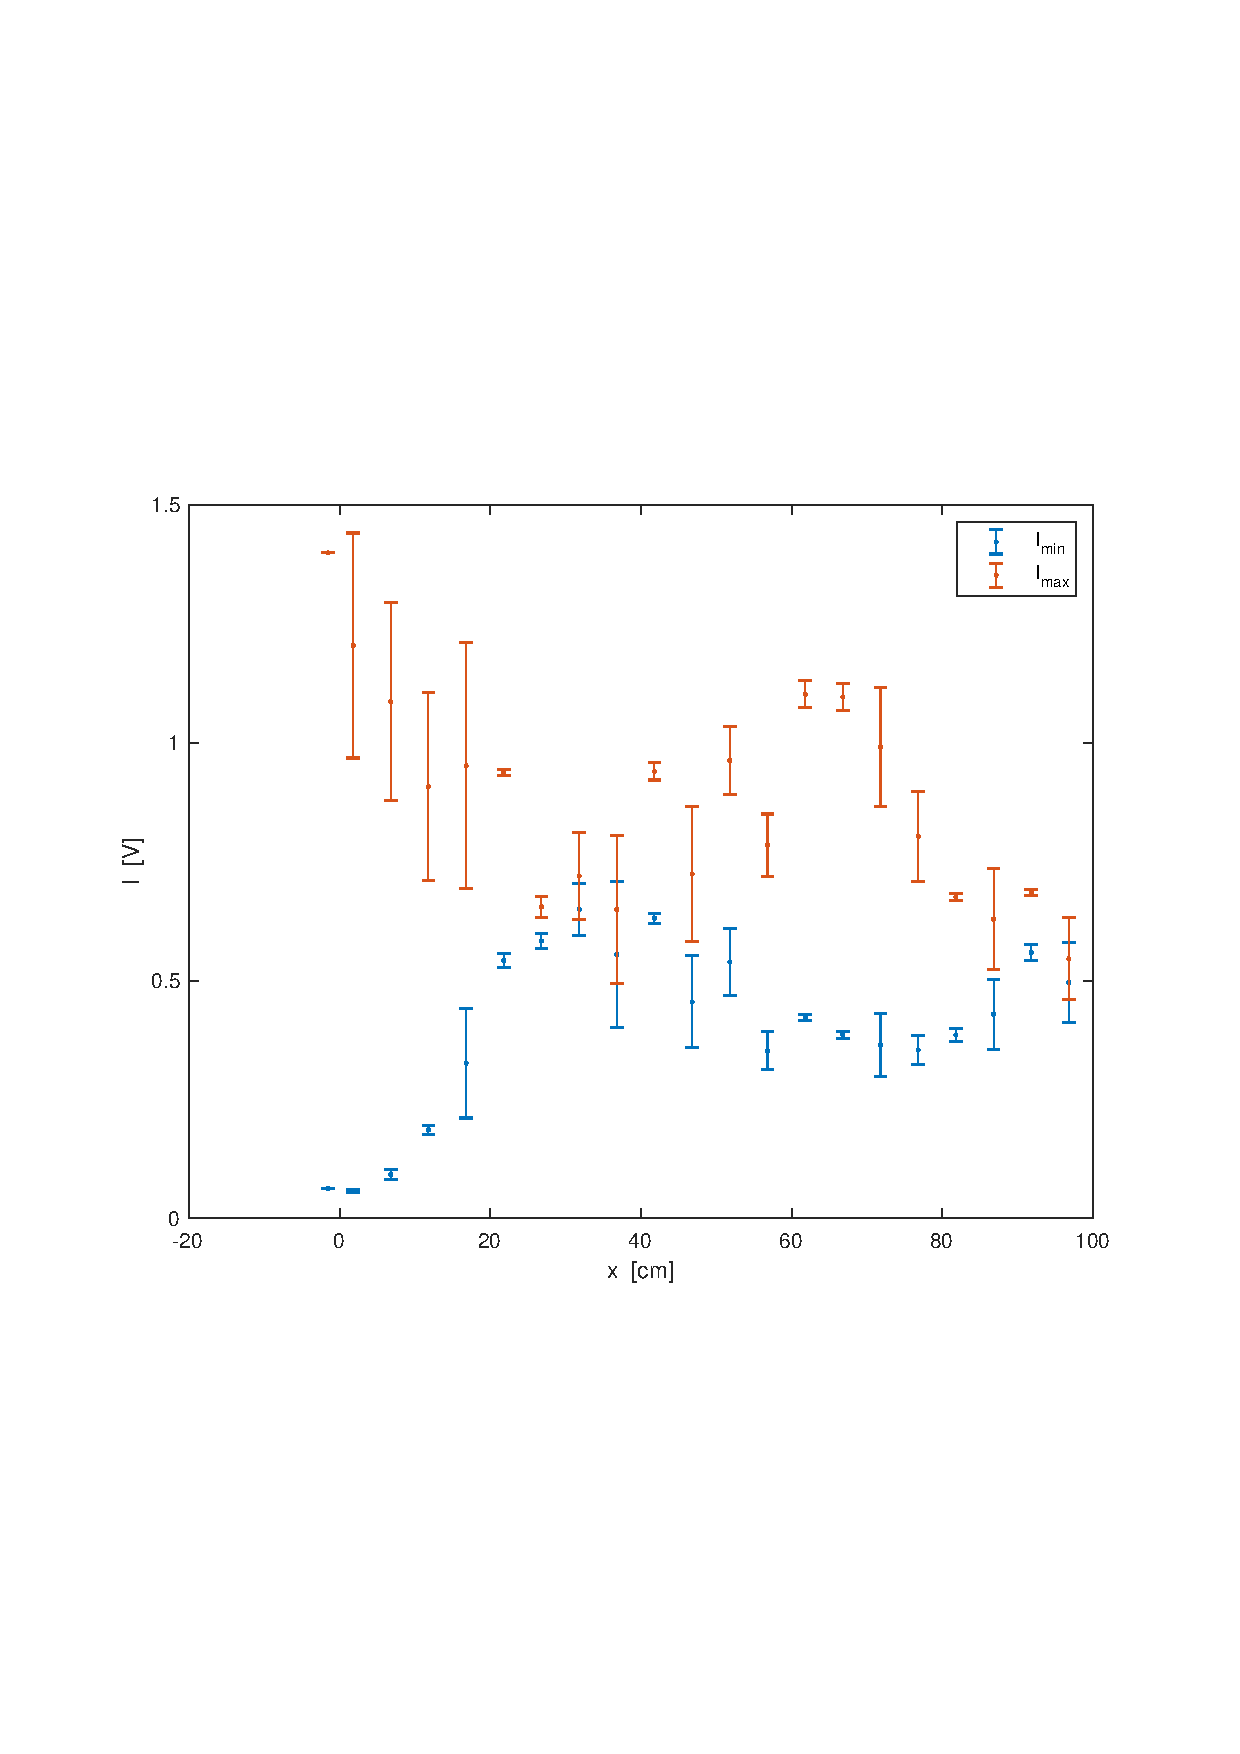
\includegraphics[width=\linewidth]{<Imax-min>_vs_tau.pdf}
	\captionof{figure}{Medie delle intensità massime e minime misurate a $x$ fissata.}
	\label{fig:averageIntensities}
	\end{center}
\end{Figure}

Si osserva come per alcuni valori dell'intensità massima la barra di errore sia molto ampia: si ritiene che questo sia dovuto ad un non corretto allineamento del fascio con l'area sensibile del fotodiodo, condizione che viene modificata ad ogni successivo aggiustamento della configurazione degli specchi.

Si riportano quindi in Figura~\ref{fig:averageVisibilities} le visibilità calcolate per ogni coppia di valori di intensità massima e minima misurati a differenza di cammino ottico fissata. Si rammenta che la visibilità è definita da
\begin{equation}\label{eq:visibility}
V = \frac{I_\text{max} - I_\text{min}}{I_\text{max} + I_\text{min}}.
\end{equation}

\begin{Figure}
	\begin{center}
	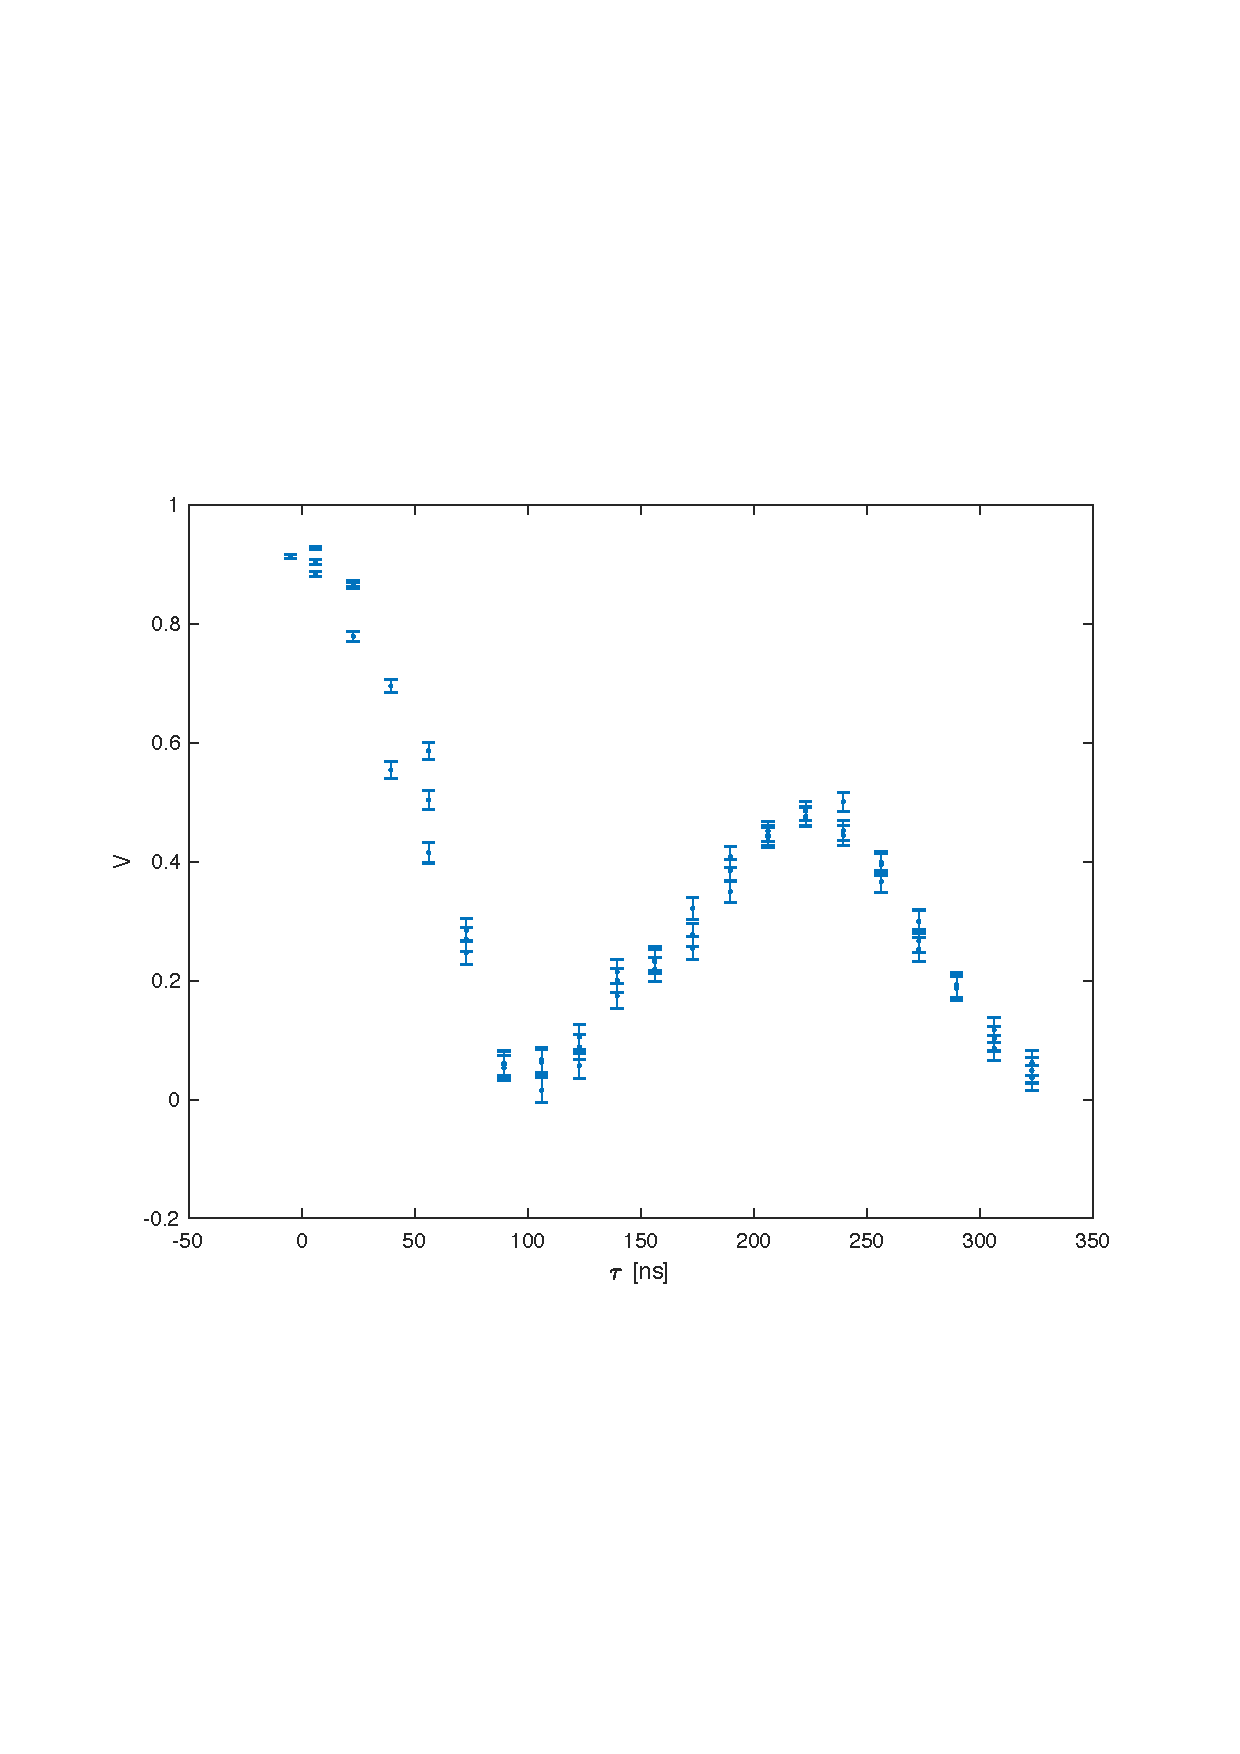
\includegraphics[width=\linewidth]{Vall_vs_tau.pdf}
	\captionof{figure}{Visibilità calcolate a $x$ fissata.}
	\label{fig:averageVisibilities}
	\end{center}
\end{Figure}

Si osserva come la scelta di acquisire tre punti sperimentali per ogni fissata distanza tra specchi e beamsplitter abbia permesso di ottenere un andamento meno disperso della visibilità: lo si confronti infatti con il grafico precedente.

In Figura~\ref{fig:visibility} è riportato il grafico della visibilità in funzione della differenza di cammino ottico, definita come 
\[
\tau = \frac{x}{c} =  \frac{d^{(0)}_\mathrm{fisso} - d(N)}{c},
\] 
dove $c$ indica la velocità della luce, $c~=~\SI{2.9979e10}{cm/s}$.

\begin{Figure}
	\begin{center}
	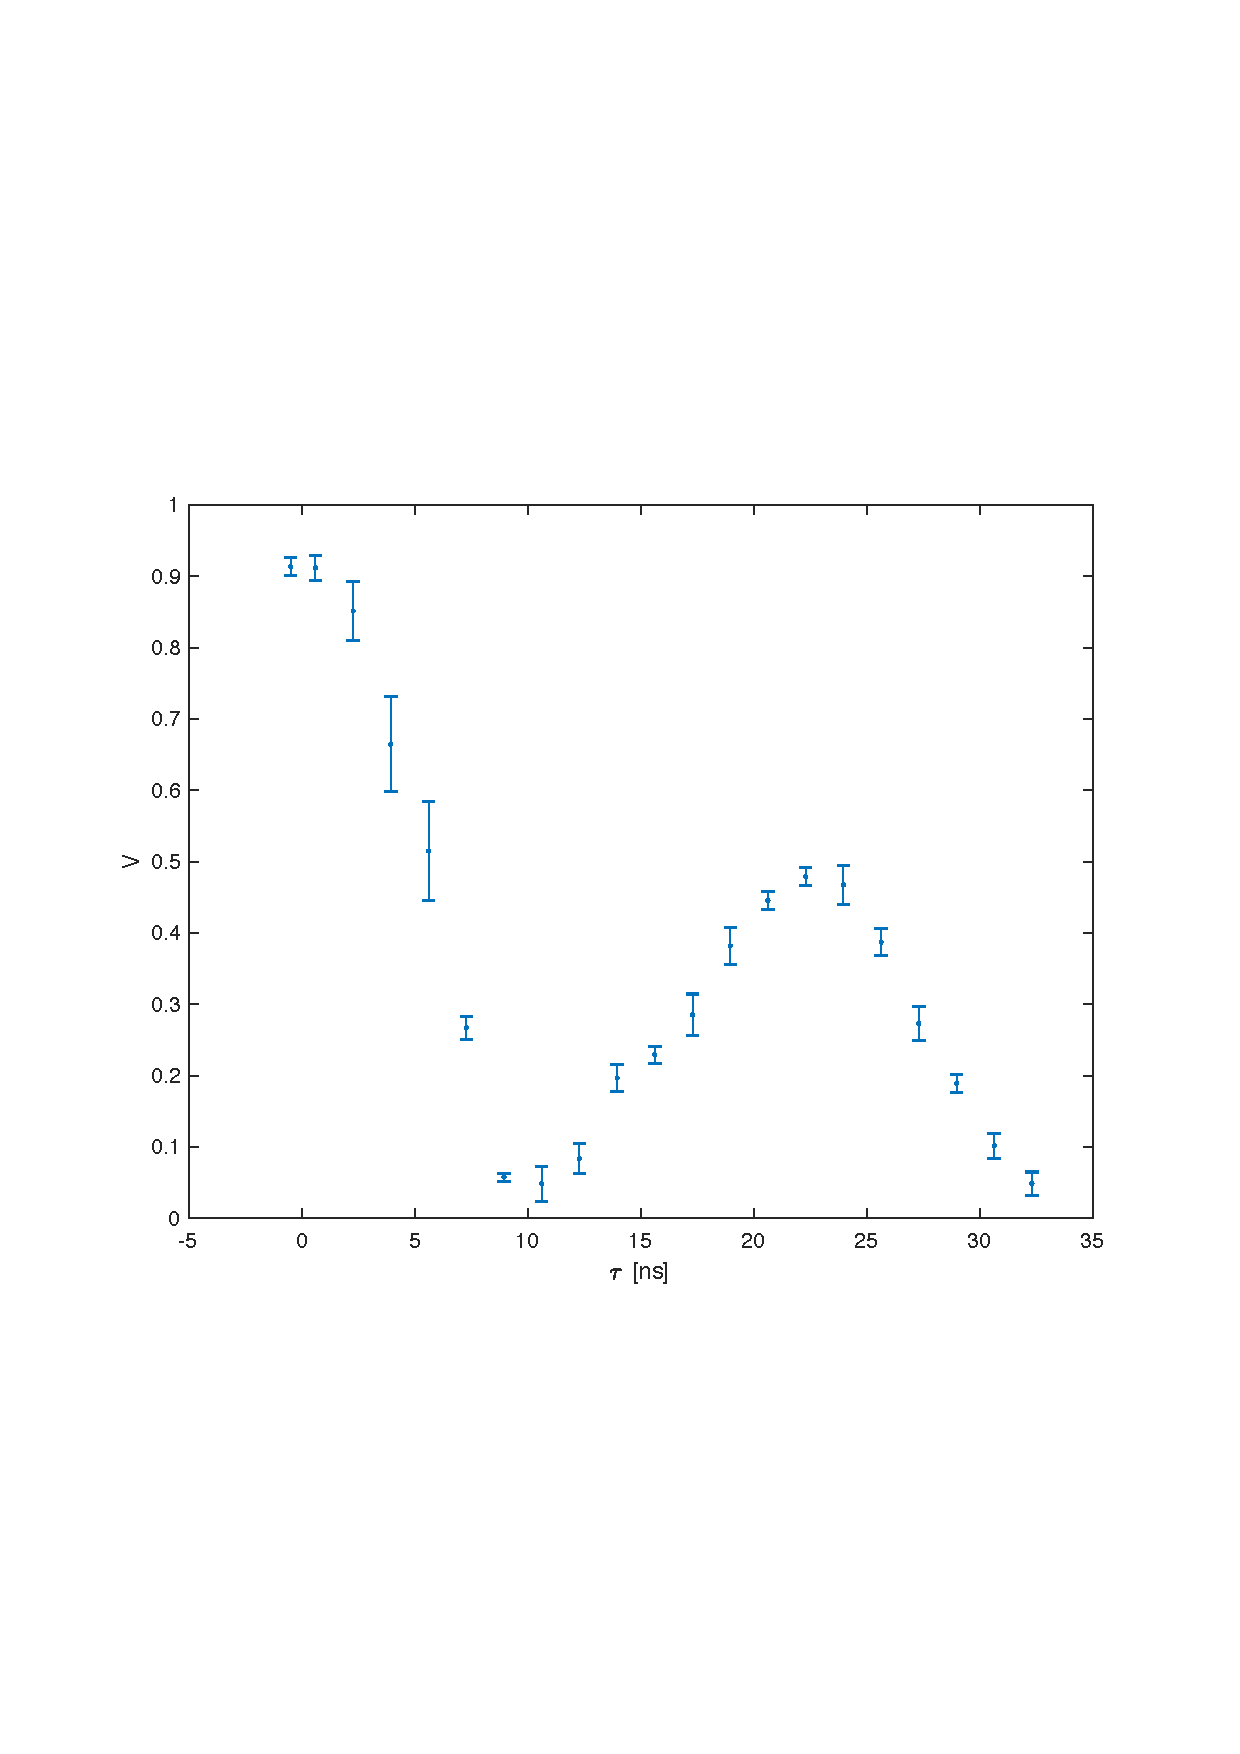
\includegraphics[width=\linewidth]{V_vs_tau.pdf}
	\captionof{figure}{Medie delle visibilità calcolate a $\tau$ fissato.}
	\label{fig:visibility}
	\end{center}
\end{Figure}

Ogni valore in funzione di $V$ è ottenuto come media pesata delle visibilità calcolate precedentemente, a partire dalle tre acquisizioni di intensità. L'incertezza associata è data dalla somma in quadratura dell'errore caratteristico della media pesata e della dispersione statistica dei tre punti sperimentali:
\[
\sigma_V = \left[ \left( \sum_{i=1}^3 \frac{1}{\sigma_\text{$V_i$}^2}\right)^{-1} + \delta(V_i)^2 \right]^{1/2}, 
\]
dove $\sigma_\text{$V_i$}$ indica l'incertezza associata a ciascun valore della visibilità dato dalla~(\ref{eq:visibility}), mentre $\delta(V_i)$ indica la dispersione statistica dei tre valori.

L'equazione (\ref{eq:visibility}) può essere riscritta in termini del modulo della funzione di correlazione $\gamma(\tau)$ e delle intensità dei due fasci ottenuti attraverso il beam-splitter:

\begin{equation}\label{eq:visibility2}
V = \frac{2\sqrt{I_1 I_2}}{\langle I_1 + I_2 \rangle}\vert \gamma(\tau) \vert
\end{equation}

Quando i fasci provengono dalla stessa sorgente $I_1=I_2$ e quindi $V = \vert\gamma(\tau)\vert$. Si esegue un fit dei dati riportati nella Figura \ref{fig:visibility} attraverso la funzione di correlazione prevista per un laser He-Ne a due modi normali di oscillazione ($N=2$):
\[
\gamma(\tau) = e^{-A\frac{\vert\tau\vert}{2}}\cos\left({B\frac{\vert\tau\vert}{2}}\right)
\]

con A e B parametri di fit. Si sottolinea che il valore di $N=2$ è stato ottenuto confrontando i dati sperimentali con le curve teoriche calcolate per $N=2$ e $N=3$, in quanto non è stato possibile eseguire un fit con anche $N$ tra i parametri liberi, a causa della divergenza del metodo dei minimi quadrati, quale è stato adoperato. Si trova
\[
\begin{aligned}
A &= \SI{0.81 \pm 0.06}{\nano\second}^{-1} \\
B &= \SI{2.79 \pm 0.06}{\nano\second}^{-1} \\
\end{aligned}
\]

Con un corrispondente R-squared pari al $95\%$. Si ricorda che R-squared è una misura percentuale della bontà del fit che raggiunge il $100\%$ quando la funzione data è in perfetto accordo con i dati sperimentali. La curva teorica sovrapposta ai dati sperimentali è riportata in figura \ref{fig:fit}. La discrepanza teoria-esperimento è più evidente in corrispondenza del secondo picco, dove l'allineamento dei due fasci è un'operazione più delicata a causa della maggiore distanza del secondo specchio.

Dalla conoscenza di A si ricava il tempo di coerenza $\tau_c$, definito come il valore per il quale $\vert\gamma\vert$ si riduce di un fattore $1/e$, escludendo l'effetto del termine oscillante. Si calcola inoltre la lunghezza di coerenza $l_c \equiv \tau_c c$. Troviamo:

$$\tau_c = \frac{2}{A} = \SI{2.5 \pm 0.2}{\ns}$$

$$l_c = \SI{74 \pm 6}{cm}$$

Confrontando i risultati ottenuti con la lunghezza di coerenza prevista dal costruttore\footnote{\url{https://www.thorlabs.com/drawings/c29db02485c2452c-B4410FB1-B1CD-8FD7-CC6F6ADA698822BC/HNL020LB-Manual.pdf}} ($l_c \simeq \SI{30}{cm}$), si osserva che i valori ottenuti sono incompatibili. Si ritiene che questo possa essere dovuto ad una diversa definizione della lunghezza di coerenza o alla presenza di sistematiche sperimentali non note (si veda la sezione successiva).\\
Il tempo di coerenza può essere definito anche come il tempo in corrispondenza del quale la funzione di correlazione si annulla per la prima volta \footnote{R.Fowles, Introduction to modern optics, ch 3.5-3.6}. Adottando questa definizione si trova
$$\tau_c = \frac{\pi}{B} = \SI{1.13 \pm 0.02}{ns}$$
$$l_c = \SI{33.9 \pm 0.6}{cm}$$
Compatibile con i valori forniti dal manuale del costruttore.


\begin{Figure}
	\begin{center}
	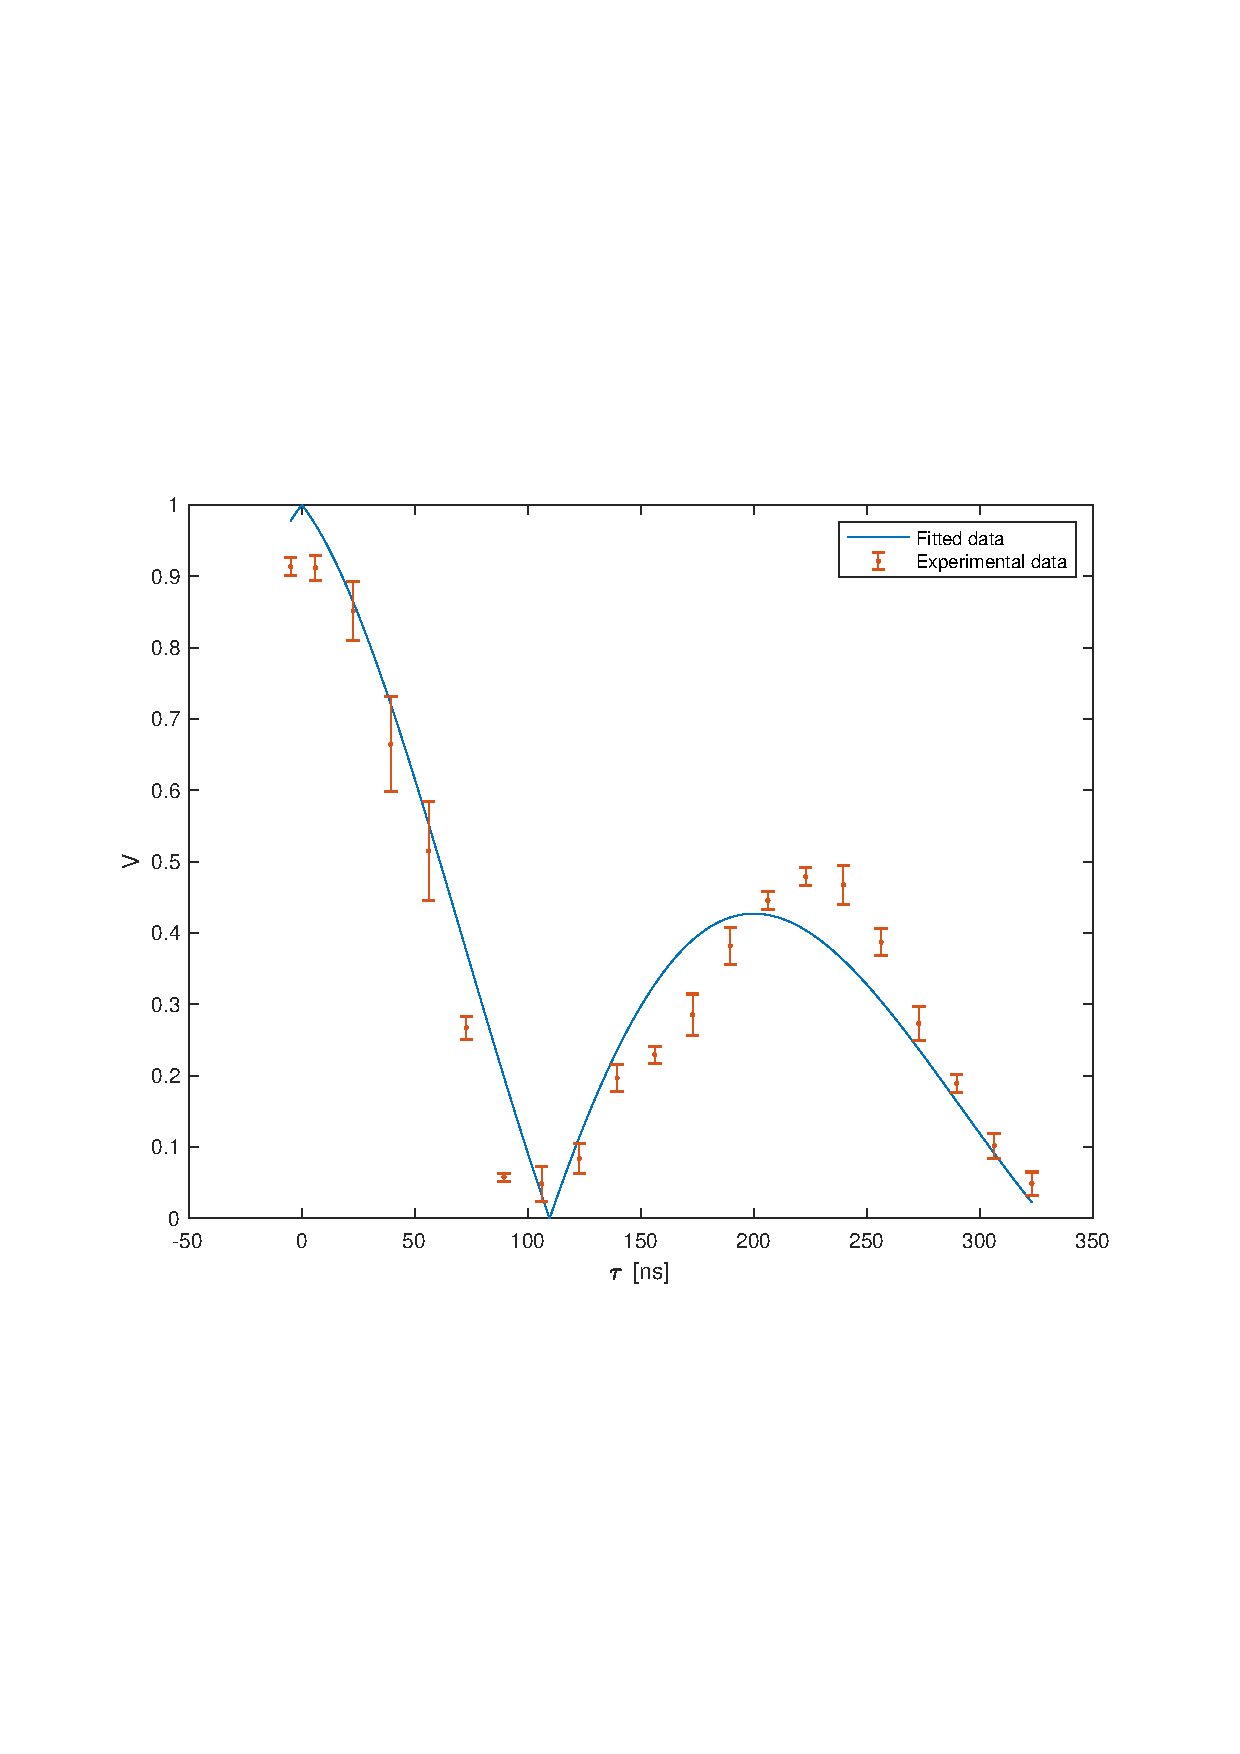
\includegraphics[width=\linewidth]{FIT.pdf}
	\captionof{figure}{Medie della visibilità per differenti valori dello sfasamento temporale tra i due fasci. Al grafico è sovrapposta la curva di fit.}
	\label{fig:fit}
	\end{center}
\end{Figure}

\section{Conclusioni}
Si ritiene che la distribuzione sperimentale dei dati, nonostante l'indicazione data dal valore di R-squared, non possa essere ragionevolmente ottenuta dal modello teorico; si osserva inoltre che le incertezze in diversi casi sono eccessivamente sottostimate, indice della presenza di sistematiche sperimentali che hanno influito sulla bontà della misura. 

Dal punto di vista dell'esecuzione, si ritiene che la non perfetta collimazione del fascio laser con l'area sensibile del fotodiodo, e altresì dei due fasci interferenti tra loro, possa aver contribuito ad alterare significativamente la distribuzione del valore atteso della visibilità. Si ipotizza che la presenza di fenomeni diffrattivi possa aver indotto a posizionare i fasci riuniti sul fotodiodo in modo non simmetrico e variabile ad ogni ricollocazione degli specchi, così da introdurre un fattore esterno a influenzare il valore della visibilità: questo è più evidente per i punti prossimi allo zero, per i quali l'incertezza minore suggerisce, in effetti, una sottostima della stessa più che una bontà del dato ottenuto. 

Il costruttore del laser non fornisce indicazioni sulla definizione adottata nel calcolo del tempo di coerenza. Utilizzando due definizioni distinte si perviene rispettivamente a un valore discordante e a un valore in accordo con quello atteso. L'adozione della prima definizione implica un errore di cui nè l'andamento qualitativo dei dati nè i risultati del fit riescono a dare conto. Si propende pertanto per l'adozione della seconda definizione.





\end{multicols}


\newpage
\section{Appendice}
\begin{center}
\captionof{table}{Misure per lo studio della funzione di mutua coerenza.}
\label{tab:Ac_differenziale}
\begin{tabular}{c|c|c|c|c|c|c|c}
$b$ [\SI{}{mV}] & rms [\SI{}{mV}] & $Imax_1$ [\SI{}{V}] & $Imax_2$ [\SI{}{V}] & $Imax_3$ [\SI{}{V}] &  $Imin_1$ [\SI{}{V}] & $Imin_2$ [\SI{}{V}] & $Imin_3$ [\SI{}{V}]  \\
  &   &  $\pm 3\%$ & $\pm 3\%$ & $\pm 3\%$ &  $\pm 3\%$ & $\pm 3\%$ & $\pm 3\%$ \\
\hline
 0.87 & 1.01 &  0.896 & 1.250 & 1.470 &  0.056 & 0.064 & 0.056 \\
 0.81 & 3.08 &  1.340 & 0.832 & 1.090 &  0.096 & 0.104 & 0.080 \\
 0.61 & 1.56 &  0.640 & 0.976 & 1.110 &  0.184 & 0.176 & 0.200 \\
 0.29 & 1.69 &  0.968 & 0.628 & 1.260 &  0.400 & 0.164 & 0.416 \\
 0.92 & 1.24 &  0.944 & 0.930 & 0.940 &  0.544 & 0.562 & 0.524 \\
 0.67 & 1.33 &  0.625 & 0.666 & 0.676 &  0.562 & 0.592 & 0.598 \\
 1.14 & 1.36 &  0.780 & 0.592 & 0.790 &  0.682 & 0.574 & 0.697 \\
 1.15 & 1.27 &  0.666 & 0.452 & 0.834 &  0.558 & 0.366 & 0.744 \\
 1.01 & 1.36 &  0.962 & 0.942 & 0.918 &  0.622 & 0.628 & 0.646 \\
 0.80 & 0.98 &  0.558 & 0.904 & 0.712 &  0.344 & 0.580 & 0.444 \\
 0.65 & 1.41 &  1.030 & 0.996 & 0.864 &  0.612 & 0.564 & 0.444 \\
 0.46 & 1.35 &  0.704 & 0.788 & 0.864 &  0.296 & 0.380 & 0.384 \\
 1.46 & 1.55 &  1.100 & 1.070 & 1.140 &  0.424 & 0.416 & 0.432 \\
 0.51 & 1.36 &  1.130 & 1.060 & 1.100 &  0.392 & 0.376 & 0.392 \\
 1.03 & 1.74 &  1.080 & 1.080 & 0.816 &  0.416 & 0.408 & 0.272 \\
 0.71 & 1.82 &  0.848 & 0.892 & 0.672 &  0.368 & 0.384 & 0.312 \\
 0.67 & 1.87 &  0.682 & 0.680 & 0.666 &  0.368 & 0.394 & 0.398 \\
 0.57 & 2.12 &  0.628 & 0.502 & 0.760 &  0.430 & 0.340 & 0.520 \\
 0.81 & 0.99 &  0.694 & 0.678 & 0.688 &  0.584 & 0.552 & 0.544 \\
 0.76 & 1.96 &  0.429 & 0.633 & 0.578 &  0.379 & 0.574 & 0.538 \\
 0.87 & 1.01 &  1.400 &	   &	        &  0.064 & 	 & 	\\
\hline
\end{tabular}
\end{center}



















%ESEMPIO DI FIGURA
%\begin{Figure}
%	\begin{center}
%	\includegraphics[width=\linewidth]{comune.png}
%	\captionof{figure}{Istantanea dell'oscilloscopio per l'amplificatore differenziale, misura di $A_c$}
%	\label{fig:Ac_differenziale}
%	\end{center}
%\end{Figure}


%ESEMPIO DI TABELLA
%\begin{center}
%\captionof{table}{Misure per la stima di $A_c$}
%\label{tab:Ac_differenziale}
%\begin{tabular}{c|c|c|c}
%$f$ [\SI{}{Hz}] & $V_i$ [\SI{}{V}] & $v_o$ [\SI{}{mV}] & $A_c = v_o / V_i$ \\
%\hline
%      149.5 &        3.90 &         11.3 & 2.90e-03 \\
%      222.0 &        3.90 &         11.5 & 2.95e-03 \\
%      281.0 &        3.90 &         11.8 & 3.03e-03 \\
%      359.0 &        3.90 &         11.8 & 3.03e-03 \\
%      461.0 &        3.90 &         12.2 & 3.13e-03 \\
%\hline
%\end{tabular}
%\end{center}


\end{document}
